\documentclass[11pt]{article}
\usepackage[textwidth=18cm,textheight=25cm]{geometry} % Edit as required


\pagestyle{empty}

% Packages
\usepackage[usenames,dvipsnames]{color} % For custom colours
\usepackage{titlesec} % For custom section headings
\usepackage{mdwlist} % For compact lists
\usepackage[pdftex]{hyperref}
\usepackage{marvosym} % For icons
\usepackage{graphicx}
\usepackage{aas_macros}
\usepackage{natbib}

\usepackage{enumitem}
\setlist{nolistsep}

\usepackage{wrapfig}

% Hyperlink colour and style
\definecolor{linkcolour}{rgb}{0,0.2,0.6}
\hypersetup{colorlinks,breaklinks, urlcolor=linkcolour, linkcolor=linkcolour}

\renewcommand{\bibsection}{\section*{Referred Publications}}
\renewcommand{\bibsep}{5pt}	% Tighten spacing between references

% Custom colour
\definecolor{lgray}{gray}{0.4}

% Custom list bullet
\renewcommand{\labelitemi}{$\succ$}

% Header commands
\newcommand{\name}[1]{\LARGE\textbf{#1}}
\newcommand{\address}[1]{\small{\color{lgray}{#1}}}
\newcommand{\tel}[1]{\small{#1}}
\newcommand{\email}[1]{\href{mailto:#1}{\small{#1}}}
\newcommand{\web}[2]{\href{#1}{\small{#2}}}
	
% Section headings
\titleformat{\section}{\large\scshape\raggedright}{}{0em}{}[\titlerule]
\titlespacing{\section}{0pt}{0.6cm}{5pt}
% Note: Create an environment for sections ?

\setlength{\parindent}{0cm}

% Full width tables
\newenvironment{ftabular}[1]
{\begin{tabular*}{0.95\textwidth}{@{\extracolsep{\fill}}#1}}
{\end{tabular*}}

\begin{document}

\vspace{-2.5in}
\begin{wrapfigure}{r}{0.10\textwidth}
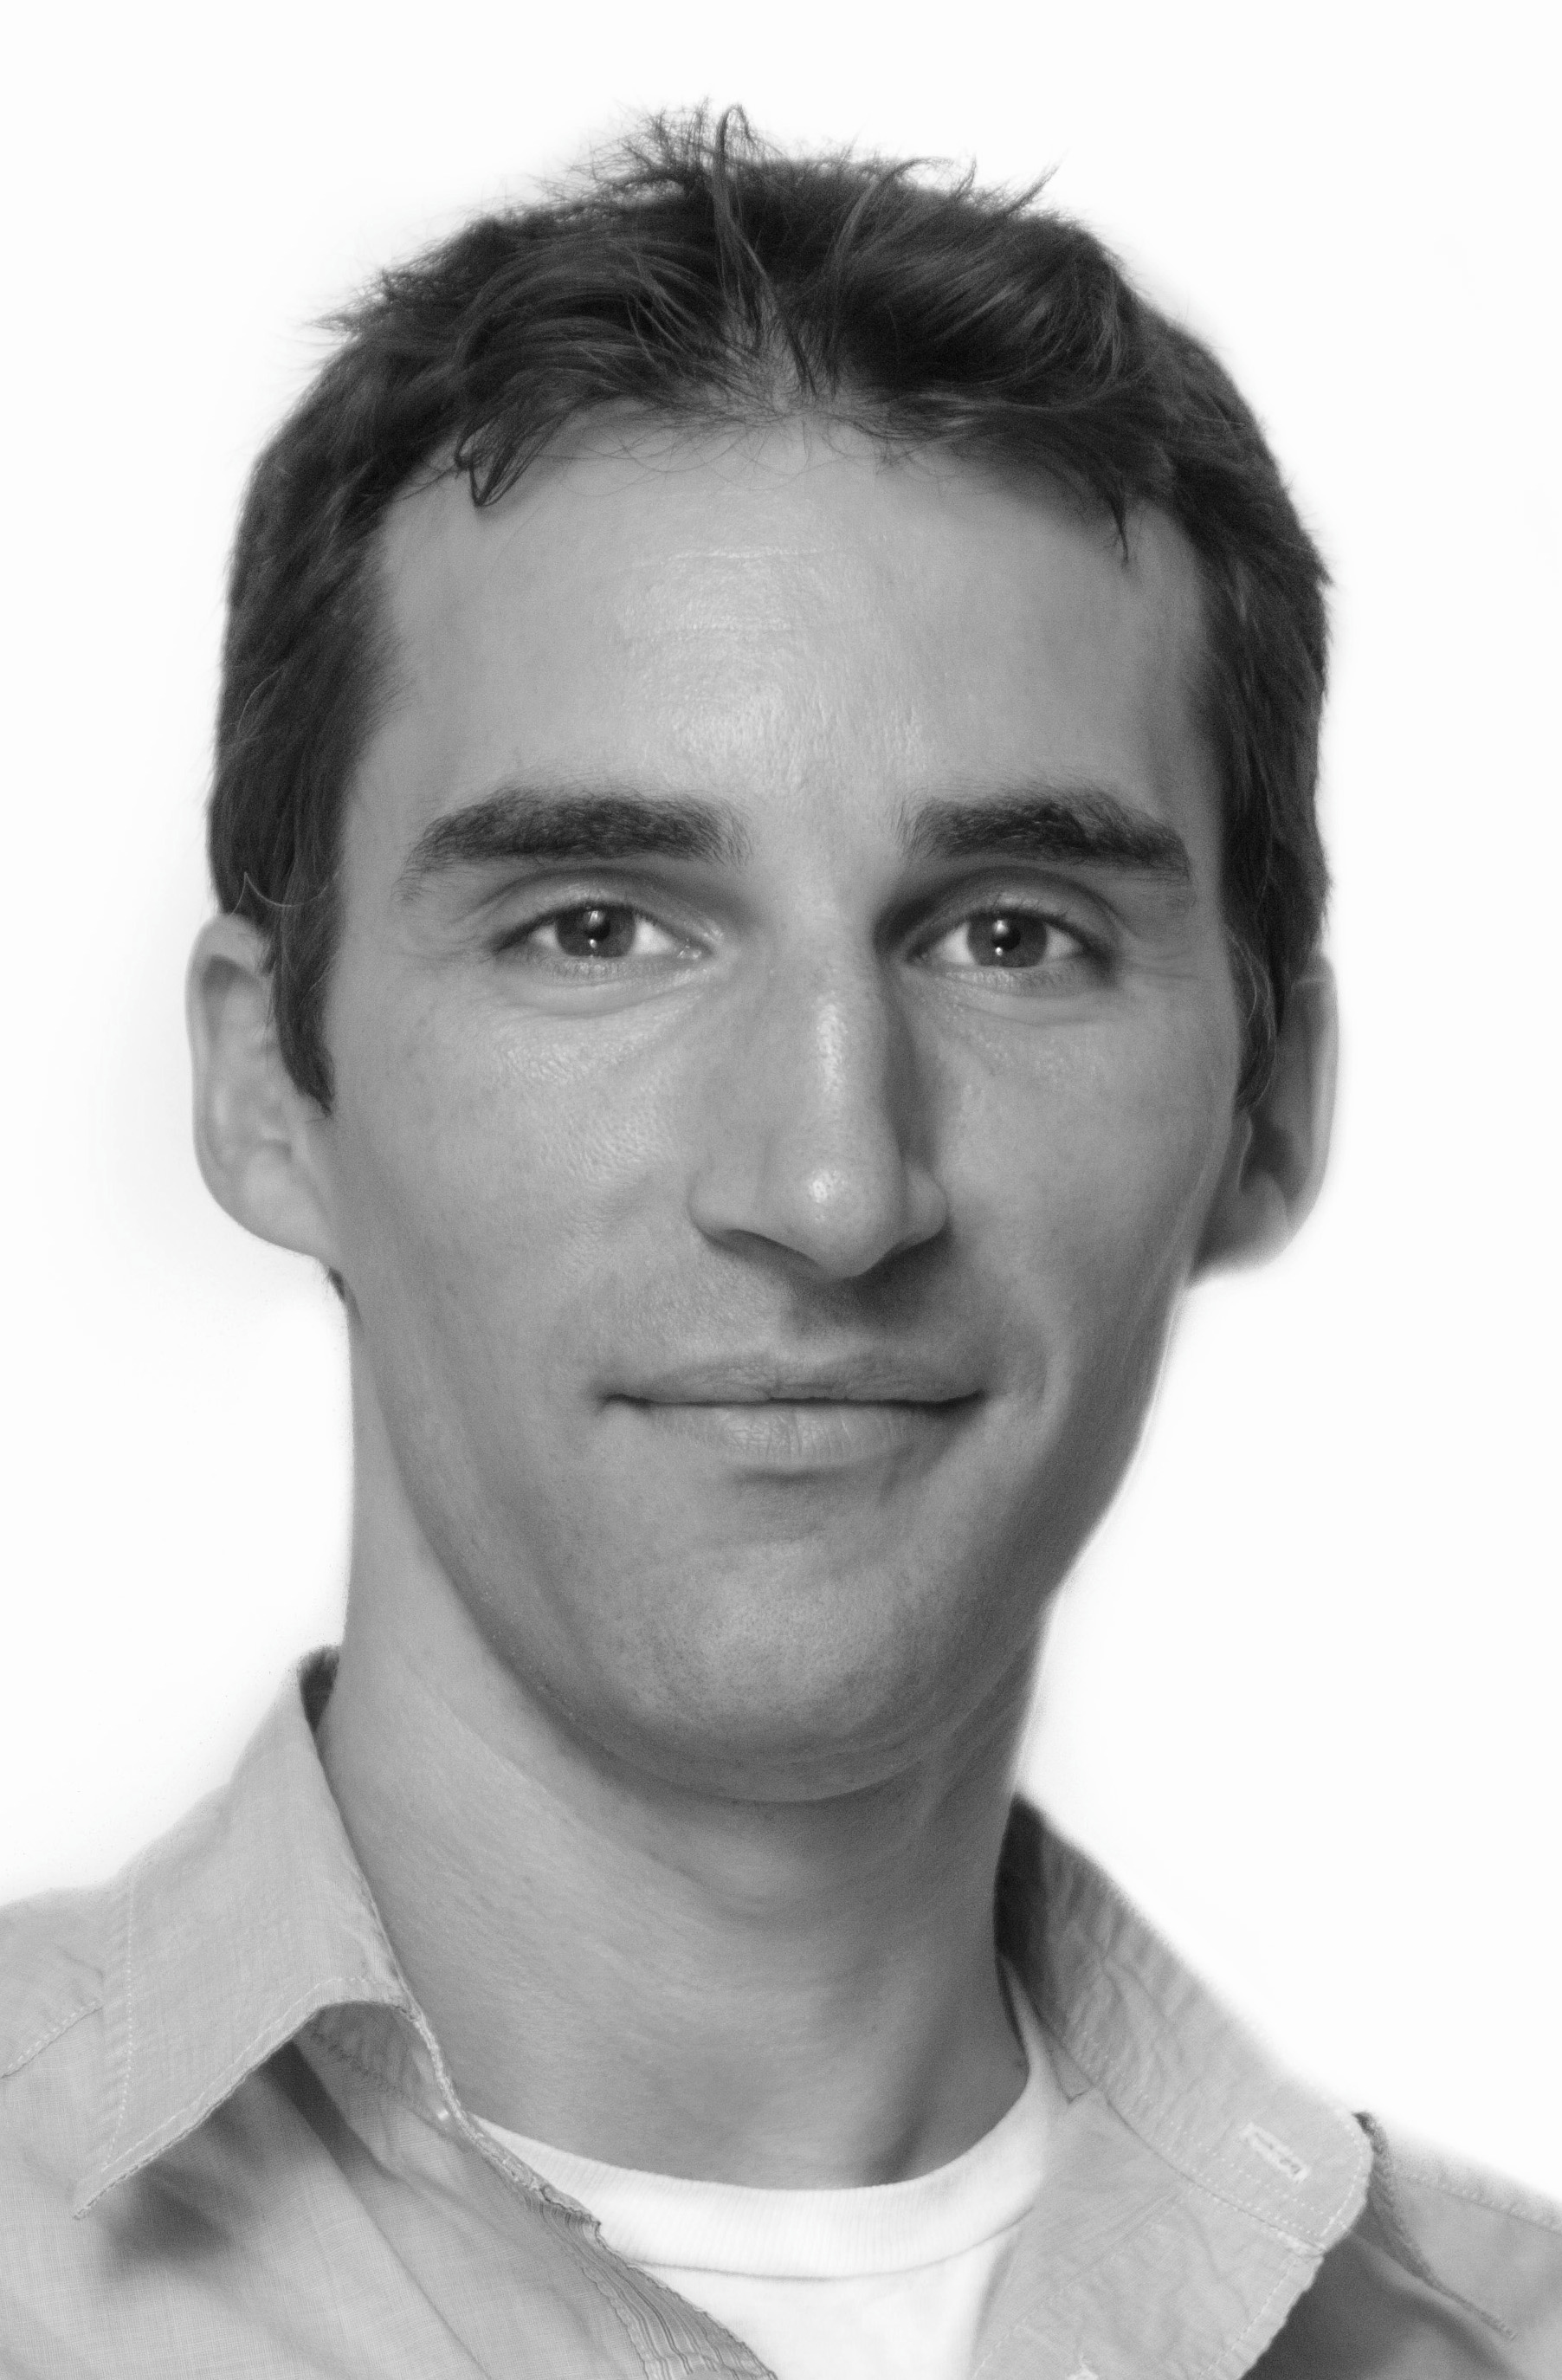
\includegraphics[width=0.09\textwidth]{mugshot.jpg}
\end{wrapfigure}


\name{Steven D. Christe, Ph.D.} \\
\address{Solar Physics Laboratory, Heliophysics Division \\
NASA Goddard Space Flight Center, Greenbelt, MD} \\
\tel{mobile: +1 510.499.0756}\\
\tel{work: +1 301.286.7999} \\
\email{schriste@cal.berkeley.edu}
% \web{http://www.example.com}{example.com}

\section{Education}
\begin{ftabular}{lr}
Ph.D. in Physics , U.C. Berkeley (Prof. R. P. Lin) & \textsc{2007}\\
B.S. in Physics, \& B.S. in Mathematics, S.U.N.Y at Stony Brook & \textsc{2001}\\
\end{ftabular}

\section{Professional Status}
\begin{ftabular}{r|p{14cm}}
\textsc{10/2009 to present} & \textbf{Research Astrophysicist, NASA Goddard Space Flight Center} \\

\multicolumn{2}{c}{ } \\ % Spacer 

\textsc{01/2008 to 10/2009} & \textbf{Post-doc, Space Sciences Laboratory, U.C. Berkeley}\\

\multicolumn{2}{c}{ } \\ % Spacer 

\textsc{09/2002 to 12/2007} & \textbf{Graduate Student, Space Sciences Laboratory, U.C. Berkeley}\end{ftabular}

\section{Professional Experience}
\begin{itemize*}
 \item PI of the HEROES balloon payload, a hard x-ray telescope for astrophysics modified to observe the Sun in addition to astrophysical targets. Led successful launch campaign in 2013. Solar observation have set a new limit on the presence of accelerated electrons in quiet active regions.
 \item Led successful launch of the FOXSI sounding rocket which applied direct imaging to solar hard x-ray observations for the first time.
  \item Spearheaded new sounding rocket proposal to apply Transition Edge Sensors to solar observations which will provide direct spectroscopic imaging with an energy resolution of 0.001\% at 3 keV.
 \item Independently developed high-sensitivity search algorithm to identify microflares in RHESSI solar
data archive. Implemented algorithm resulting in largest database of its kind.
 \item Designed novel solar X-ray focusing optics telescope through collaboration with the Marshall Space Flight Center and the Japanese Aerospace Exploration Agency.
 \item Raised a total of \$5.7M in funding from NASA proposals over 6 years.
 \item Developed solar hard x-ray telescope instrument concept which was included in 3 concept missions proposed to the Heliophysics Decadal Survey. Presented invited talk at Panel discussion.
 \item Given over 65 presentations at international conferences and workshops .
 % 10th rhessi workshop, 12th rhessi workshop, MTSSC
 \item Served on scientific organizing committee for several international workshops.
\end{itemize*} 

\section{Teaching, Mentoring, \& Community Service}
\begin{itemize*}
\item Developed curricula and lectures for presentation in discussion sections of university-level introductory physics courses. Led discussion and physics-lab sections for physics courses with up to approximately 200 students.
% Emily Rauscher, Natsuha Kuroda, Alex Cramer, Marcello Rodriguez, Kyle Gregory, Robert Taylor, +1, Lindsay Glesener, Paula, Simon, 
\item Mentored over 15 students leading to over 10 presentations at international conferences and workshops.
\item Founding member and Chair of the SunPy organization whose mission is to develop SunPy, a community-developed, free and open-source solar data analysis environment for Python (\url{sunpy.org}). Has over 20k lines of code by over 40 contributors.
\item Established, designed, implemented, and maintained the \href{http://sprg.ssl.berkeley.edu/~tohban/wiki/index.php/RHESSI_Science_Nuggets}{RHESSI Science Nuggets website}, a successful community website for solar astrophysics research news. Hosts over 230 articles by over 120 authors from across the solar physics community.
\item Raised over \$50k to support international student participation in the SunPy project from the \href{https://developers.google.com/open-source/soc/}{Google Summer of Code} and the \href{http://sophia.estec.esa.int/socis2014/}{ESA Summer of Code} programs.
\end{itemize*}

\section{Awards, Honors, \& Professional Societies}
\begin{itemize*}
\item GSFC Special Act - Individual Award
\item Member of American Geophysical Union, American Astronomical Society
\item \href{https://jsi.astro.umd.edu}{Joint Space Institute Fellow}
\item NASA Early Career Scientist and Engineer Working Group
\end{itemize*}
\nocite{*}
\bibliographystyle{humannat}
\bibliography{publications}

\end{document}

